\documentclass[aspectratio=149]{beamer}


\usepackage{lmodern}
\usepackage{amsmath}
\usepackage{hyperref}
\usepackage{booktabs}
\usepackage{url}
\usepackage{smartdiagram}
\usepackage{bm}
\usepackage{csquotes}
\usepackage{graphicx}
\usepackage[utf8]{inputenc}
\usepackage{amsmath}
\usepackage{lipsum}
\usepackage{float}
\usepackage{textgreek}
\usepackage{tikz}
\usepackage{datetime}
\usepackage[backend=bibtex,style=authoryear]{biblatex}
\usepackage{listings}
\usepackage{setspace}
\usepackage{braket}
\usepackage[font=small,format=plain,labelfont=bf,up,textfont=normal,up,format=hang]{caption}

\usepackage{tikz}
\usetikzlibrary{shapes.geometric, arrows}

\usecolortheme{crane}

\tikzstyle{startstop} = [rectangle, rounded corners, minimum width=3cm, minimum height=1cm,text centered, draw=black, fill=red!30]
\tikzstyle{io} = [trapezium, trapezium left angle=70, trapezium right angle=110, minimum width=3cm, minimum height=1cm, text centered, draw=black, fill=blue!30]
\tikzstyle{process} = [rectangle, minimum width=3cm, minimum height=1cm, text centered, draw=black, fill=orange!30]
\tikzstyle{decision} = [diamond, minimum width=3cm, minimum height=1cm, text centered, draw=black, fill=green!30]
\tikzstyle{arrow} = [thick,->,>=stealth]

\addbibresource{ref.bib}

\newdateformat{monthyeardate}{\footnotesize \monthname[\THEMONTH], \THEYEAR}
\title{Face Detection, Recognition and Tracking}
\author[Pawan]{\texorpdfstring{\\}{}
    Pawan Singh Negi \- \texorpdfstring{$174010003$}{}  \texorpdfstring{\\}{}
    Aarif Shaikh \- \texorpdfstring{$173310007$}{}  \texorpdfstring{\\}{}
    M Kartheek \- \texorpdfstring{$163100065$}{}  \texorpdfstring{\\}{}
}

\institute[IITB]{Indian Institute of Technology, Bombay}


\begin{document}

\monthyeardate{}
\maketitle

%%%%%%%%%%%%%%%%%%%%%%%%%%%%%%%%%%%%

\begin{frame}
    \frametitle{Motivation}
    \begin{itemize}
        \item Face recognition - a very demanding technology.
        \item It needs to be fast and accurate.
        \item Very high resolution videos very common
    \end{itemize}
\end{frame}

%%%%%%%%%%%%%%%%%%%%%%%%%%%%%%%%%%%%

%%%%%%%%%%%%%%%%%%%%%%%%%%%%%%%%%%%%

\begin{frame}
\frametitle{Introduction}
\begin{itemize}
	\item Used OpenCV library
	\item Both serial and parallel code were compared.
	\item Comparison between various algorithm 
\end{itemize}
\end{frame}

%%%%%%%%%%%%%%%%%%%%%%%%%%%%%%%%%%%%

\begin{frame}
\frametitle{Overall flow of the Process}
\begin{figure}
	\centering
	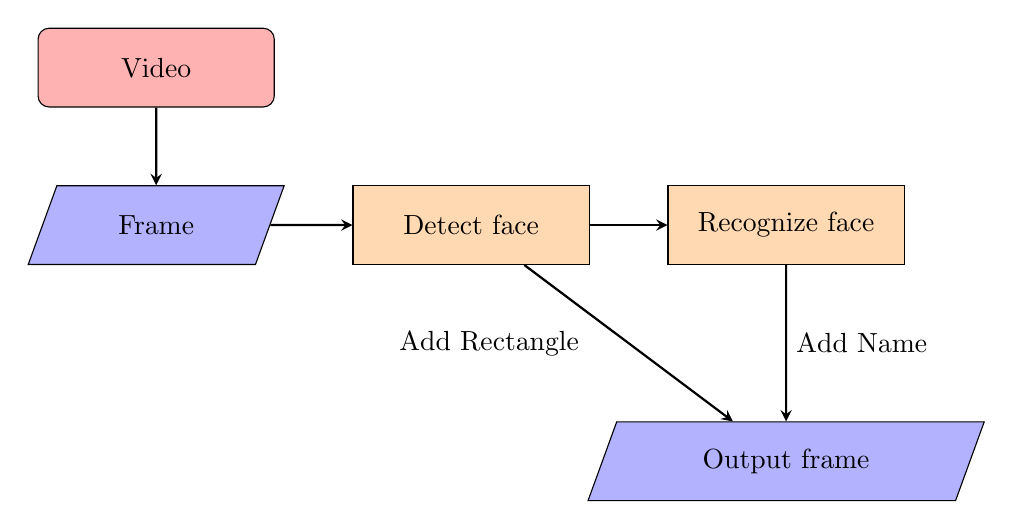
\begin{tikzpicture}[node distance=2cm]
	
	\node (start) [startstop] {Video};
	\node (frame) [io, below of=start] {Frame};
	\node (detect) [process, right of=frame, xshift=2cm] {Detect face};
	\node (recognize) [process, right of=detect, xshift=2cm] {Recognize face};
	\node (outframe) [io, below of=recognize , yshift=-1cm] {Output frame};
	
	\draw [arrow] (start) -- (frame);
	\draw [arrow] (frame) -- (detect);
	\draw [arrow] (detect) -- (recognize);
	\draw [arrow] (detect) -- node[anchor=east , xshift=-0.5cm] {Add Rectangle} (outframe);
	\draw [arrow] (recognize) -- node[anchor=west] {Add Name} (outframe);
	
	\end{tikzpicture}
	\caption{Flowchart}
\end{figure}
	
\end{frame}

%%%%%%%%%%%%%%%%%%%%%%%%%%%%%%%%%%%%
%%%%%%%%%%%%%%%%%%%%%%%%%%%%%%%%%%%%

\begin{frame}
\frametitle{Face Detection}
\resizebox{12cm}{1cm}{
	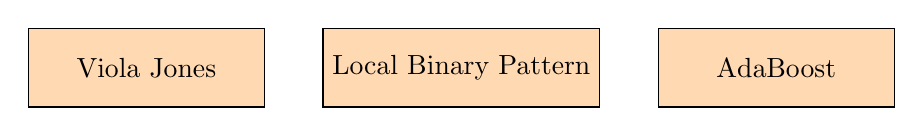
\begin{tikzpicture}[node distance=2cm]
	\node (bc) [process] {Viola Jones};
	\node (approx) [process, right of=bc,xshift=2cm] {Local Binary Pattern};
	\node (gde) [process, right of=approx, xshift=2cm ] {AdaBoost};
	\end{tikzpicture}
}
\begin{columns}
	\begin{column}{.35\textwidth}
		
	\end{column}
	\begin{column}{.35\textwidth}
		
	\end{column}
	\begin{column}{.35\textwidth}
		
	\end{column}
\end{columns} 
\footnotetext[1]{\cite{facedet}}
\end{frame}

%%%%%%%%%%%%%%%%%%%%%%%%%%%%%%%%%%%%

\begin{frame}
\frametitle{Face Detection}
\resizebox{12cm}{1cm}{
	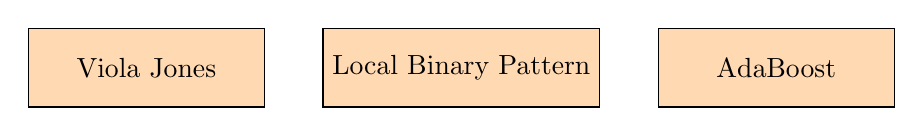
\begin{tikzpicture}[node distance=2cm]
	\node (bc) [process] {Viola Jones};
	\node (approx) [process, right of=bc,xshift=2cm] {Local Binary Pattern};
	\node (gde) [process, right of=approx, xshift=2cm ] {AdaBoost};
	\end{tikzpicture}
}
\begin{columns}
	\begin{column}{.35\textwidth}
		\begin{itemize}
			\item Highly accurate
		    \item Very fast
		    \item Long training time
		    \item Limited head poses
		    \item Cannot detect black faces
	    \end{itemize}
	\end{column}
	\begin{column}{.35\textwidth}
		
	\end{column}
	\begin{column}{.35\textwidth}
		
	\end{column}
\end{columns} 

\end{frame}

%%%%%%%%%%%%%%%%%%%%%%%%%%%%%%%%%%%%

\begin{frame}
\frametitle{Face Detection}
\resizebox{12cm}{1cm}{
	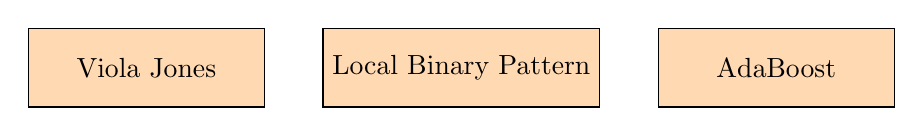
\begin{tikzpicture}[node distance=2cm]
	\node (bc) [process] {Viola Jones};
	\node (approx) [process, right of=bc,xshift=2cm] {Local Binary Pattern};
	\node (gde) [process, right of=approx, xshift=2cm ] {AdaBoost};
	\end{tikzpicture}
}
\begin{columns}
	\begin{column}{.35\textwidth}
		\begin{itemize}
			\item Highly accurate
			\item Very fast
			\item Long training time
			\item Limited head poses
			\item Cannot detect black faces
		\end{itemize}
	\end{column}
	\begin{column}{.35\textwidth}
		\begin{itemize}
			\item Detects texture
			\item Tracks movement 
			\item Easy to implement
			\item Not accurate
			\item Not recommended for RGB image		
		\end{itemize}
	\end{column}
	\begin{column}{.35\textwidth}
		
	\end{column}
\end{columns} 

\end{frame}

%%%%%%%%%%%%%%%%%%%%%%%%%%%%%%%%%%%%

\begin{frame}
\frametitle{Face Detection}
\resizebox{12cm}{1cm}{
	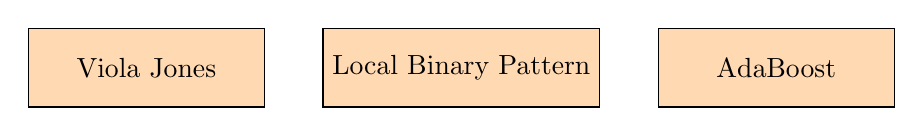
\begin{tikzpicture}[node distance=2cm]
	\node (bc) [process] {Viola Jones};
	\node (approx) [process, right of=bc,xshift=2cm] {Local Binary Pattern};
	\node (gde) [process, right of=approx, xshift=2cm ] {AdaBoost};
	\end{tikzpicture}
}
\begin{columns}
	\begin{column}{.35\textwidth}
		\begin{itemize}
			\item Highly accurate
			\item Very fast
			\item Long training time
			\item Limited head poses
			\item Cannot detect black faces
		\end{itemize}
	\end{column}
	\begin{column}{.35\textwidth}
		\begin{itemize}
			\item Detects texture
			\item Tracks movement 
			\item Easy to implement
			\item Not accurate
			\item Not recommended for RGB image		
		\end{itemize}
	\end{column}
	\begin{column}{.35\textwidth}
		\begin{itemize}
			\item Sensitive to noisy data
			\item Adaptive
			\item Simple implementation
			\item Very slow to train		
		\end{itemize}
	\end{column}
\end{columns} 

\end{frame}

%%%%%%%%%%%%%%%%%%%%%%%%%%%%%%%%%%%%

\begin{frame}
\frametitle{More on Voila Jones}
\begin{itemize}
	\item We used Voila Jones for detection.
	\item It is fast and accurate
	\item A cascade of classifiers can be built
	\item Haar Cascading is used 
\end{itemize}
\end{frame}

%%%%%%%%%%%%%%%%%%%%%%%%%%%%%%%%%%%%

\begin{frame}
\frametitle{Face Recognition}
\resizebox{12cm}{1cm}{
	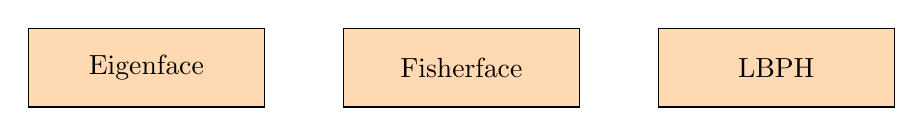
\begin{tikzpicture}[node distance=2cm]
	\node (bc) [process] {Eigenface};
	\node (approx) [process, right of=bc,xshift=2cm] {Fisherface};
	\node (gde) [process, right of=approx, xshift=2cm ] {LBPH};
	\end{tikzpicture}
}
\begin{columns}
	\begin{column}{.35\textwidth}
		
	\end{column}
	\begin{column}{.35\textwidth}
		
	\end{column}
	\begin{column}{.35\textwidth}
		
	\end{column}
\end{columns} 
\footnotetext[1]{\cite{facerec}}
\end{frame}

%%%%%%%%%%%%%%%%%%%%%%%%%%%%%%%%%%%%

\begin{frame}
\frametitle{Face Recognition}
\resizebox{12cm}{1cm}{
	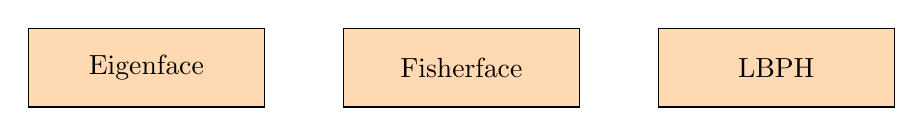
\begin{tikzpicture}[node distance=2cm]
	\node (bc) [process] {Eigenface};
	\node (approx) [process, right of=bc,xshift=2cm] {Fisherface};
	\node (gde) [process, right of=approx, xshift=2cm ] {LBPH};
	\end{tikzpicture}
}
\begin{columns}
	\begin{column}{.35\textwidth}
		\begin{itemize}
			\item Principal component analysis
			\item Maximizes total variance
			\item Any face can be represented as linear combination of these models.
			\item Distance measure criteria
		\end{itemize}
	\end{column}
	\begin{column}{.35\textwidth}
		
	\end{column}
	\begin{column}{.35\textwidth}
		
	\end{column}
\end{columns} 

\end{frame}

%%%%%%%%%%%%%%%%%%%%%%%%%%%%%%%%%%%%

\begin{frame}
\frametitle{Face Recognition}
\resizebox{12cm}{1cm}{
	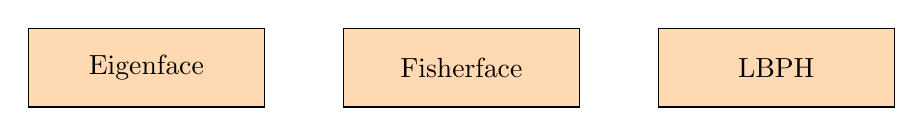
\begin{tikzpicture}[node distance=2cm]
	\node (bc) [process] {Eigenface};
	\node (approx) [process, right of=bc,xshift=2cm] {Fisherface};
	\node (gde) [process, right of=approx, xshift=2cm ] {LBPH};
	\end{tikzpicture}
}
\begin{columns}
	\begin{column}{.35\textwidth}
		\begin{itemize}
			\item Principal component analysis
			\item Maximizes total variance
			\item Any face can be represented as linear combination of these models.
			\item Distance measure criteria
		\end{itemize}
	\end{column}
	\begin{column}{.35\textwidth}
		\begin{itemize}
			\item Linear Discriminant Analysis 
			\item Maximize ratio of the ratio of between-classes to within-classes variance
			\item More accurate
		\end{itemize}
	\end{column}
	\begin{column}{.35\textwidth}
		
	\end{column}
\end{columns} 

\end{frame}

%%%%%%%%%%%%%%%%%%%%%%%%%%%%%%%%%%%%

\begin{frame}
\frametitle{Face Recognition}
\resizebox{12cm}{1cm}{
	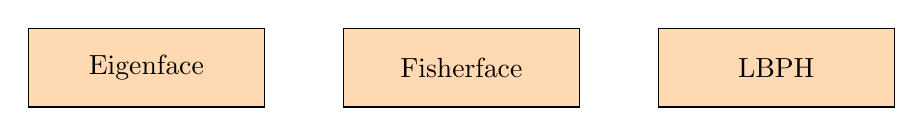
\begin{tikzpicture}[node distance=2cm]
	\node (bc) [process] {Eigenface};
	\node (approx) [process, right of=bc,xshift=2cm] {Fisherface};
	\node (gde) [process, right of=approx, xshift=2cm ] {LBPH};
	\end{tikzpicture}
}
\begin{columns}
	\begin{column}{.35\textwidth}
		\begin{itemize}
			\item Principal component analysis
			\item Maximizes total variance
			\item Any face can be represented as linear combination of these models.
			\item Distance measure criteria
		\end{itemize}
	\end{column}
	\begin{column}{.35\textwidth}
		\begin{itemize}
			\item Linear Discriminant Analysis 
			\item Maximize ratio of the ratio of between-classes to within-classes variance
			\item More accurate
		\end{itemize}
	\end{column}
	\begin{column}{.35\textwidth}
		\begin{itemize}
			\item Local binary patterns Histogram
			\item Grayscale image - each pixel are given binary digit based on neighbours 
			\item Unaffected by variance
		\end{itemize}
	\end{column}
\end{columns} 

\end{frame}

%%%%%%%%%%%%%%%%%%%%%%%%%%%%%%%%%%%%

\begin{frame}
\frametitle{Results}
\begin{figure}
	\centering
	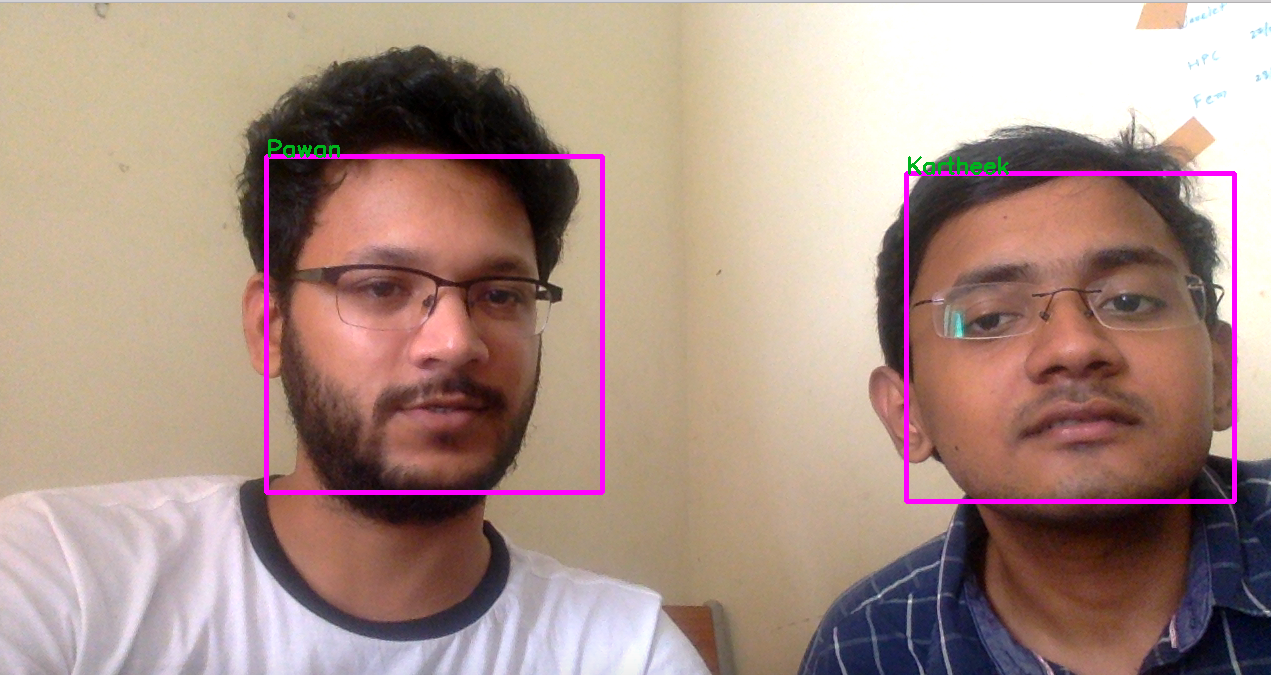
\includegraphics[scale=0.25]{./images/res.png}
	\caption{Result from Our software using Opencv}
\end{figure}
\end{frame}

%%%%%%%%%%%%%%%%%%%%%%%%%%%%%%%%%%%%

\begin{frame}
\frametitle{Speed-up}
\begin{itemize}
	\item For multiple faces needed speed.
	\item OpenCV provides two Mat definition
	\item Mat do not use GPU.
	\item UMat uses GPU.
	\item Wrote function templates to handle both.
	\item Made necessary conversion Mat$<->$UMat.
\end{itemize}
\end{frame}

%%%%%%%%%%%%%%%%%%%%%%%%%%%%%%%%%%%%

\begin{frame}
\frametitle{Multiple faces}
\begin{figure}
	\centering
	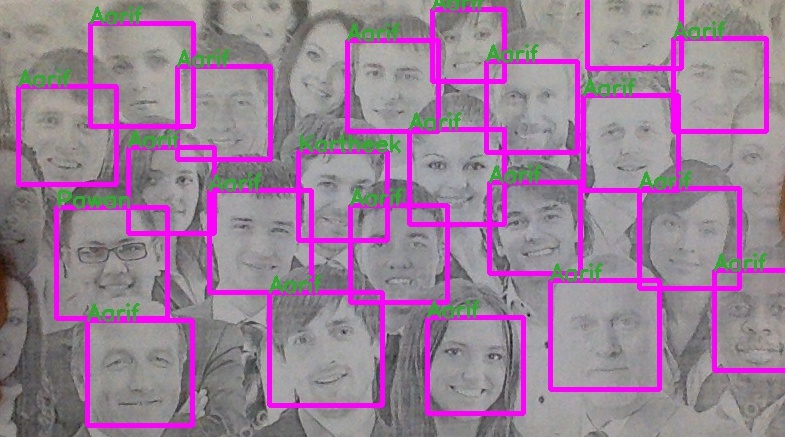
\includegraphics[scale=0.4]{./images/mul.jpg}
	\caption{Detecting Multiple faces}
\end{figure}
\end{frame}

%%%%%%%%%%%%%%%%%%%%%%%%%%%%%%%%%%%%

\begin{frame}
\frametitle{Time Study}
\begin{figure}
	\centering
	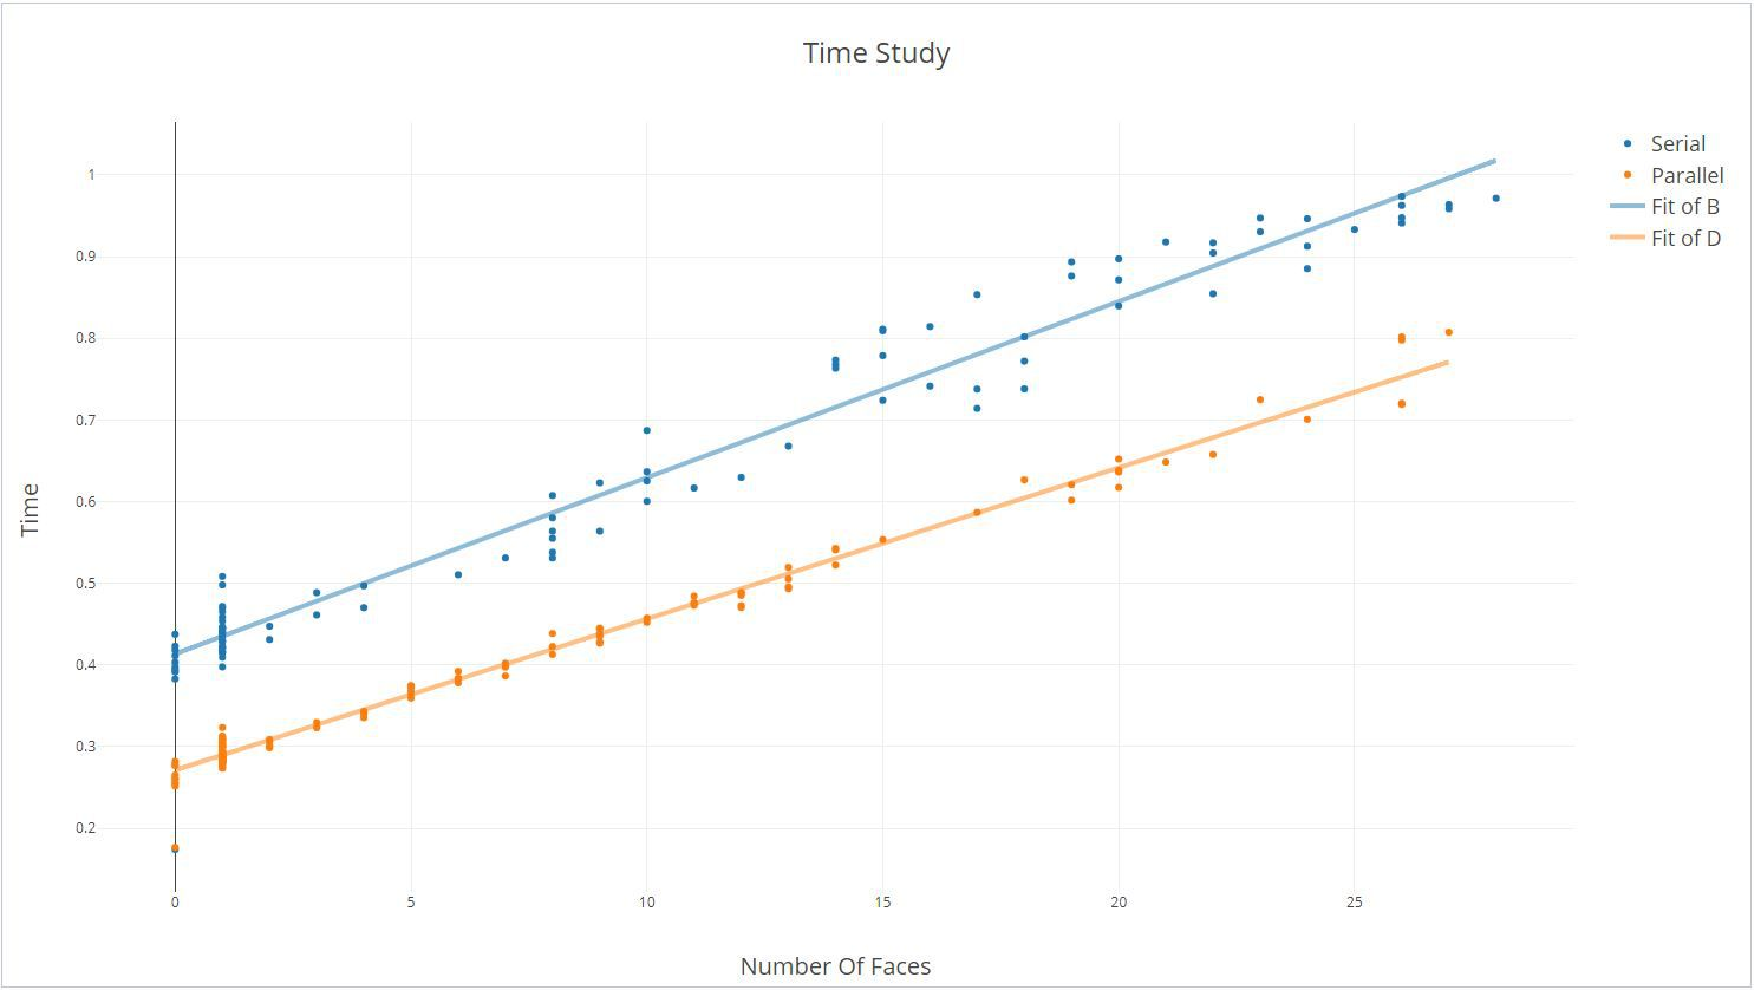
\includegraphics[scale=0.4]{./images/plot.pdf}
	\caption{Time vs Number of faces}
\end{figure}
\end{frame}

%%%%%%%%%%%%%%%%%%%%%%%%%%%%%%%%%%%%

\begin{frame}
\frametitle{Some attempts for speed-up}
\begin{itemize}
	\item Attempted tracking faces
	\item flow was as follows:
	\begin{itemize}
		\item Detect eye
		\item Calculate rotation
		\item Rotate frame
		\item Detect face
		\item Track face...
	\end{itemize}	
\end{itemize}
\footnotetext[1]{\cite{facetrack}}
\end{frame}

%%%%%%%%%%%%%%%%%%%%%%%%%%%%%%%%%%%%

\begin{frame}
\frametitle{Some course related stuff}
\begin{itemize}
	\item Used Github for version control - \url{https://github.com/psnbaba/HPC_project}
	\item Used doxygen for documentation	
\end{itemize}
\end{frame}

%%%%%%%%%%%%%%%%%%%%%%%%%%%%%%%%%%%%

\begin{frame}
\frametitle{Summary}
\begin{itemize}
	\item Used OpenCV for face detection and recognition.
	\item Face detection and recognition was parallelized.
	\item Other software taught in course used
	\item Face tracking was attempted for more speed-up	
\end{itemize}
\end{frame}

%%%%%%%%%%%%%%%%%%%%%%%%%%%%%%%%%%%%

\begin{frame}
    \centering
    Thank you
\end{frame}

\begin{frame}[t,allowframebreaks]
  \frametitle{References}
  \printbibliography{}
\end{frame}


%%%%%%%%%%%%%%%%%%%%%%%%%%%%%%%%%%%%

\end{document}
%%% Local Variables:
%%% mode: latex
%%% TeX-master: t
%%% End:
